\chapter{Хэрэгжүүлэлт}
\section{Frontend}
Хэрэглэгчийн интерфейсийг NEXTjs болон MUI сангийн тусламжтайгаар хэрэгжүүлсэн бөгөөд нэвтрэх логик болон ажиллах явцын логикуудыг хэрэгжүүлсэн билээ. Google, Github-ыг ашиглан нэвтрэх, өөрөө бүртгэл үүсгэн нэвтрэх, route-үүдийг хамгаалах, middleware-ийг хэрэгжүүлэх, сервер талдаа хүсэлт явуулах зэрэг ажлуудыг хэрэгжүүлээд байгаа билээ. 

\begin{figure}[h]
  \centering
  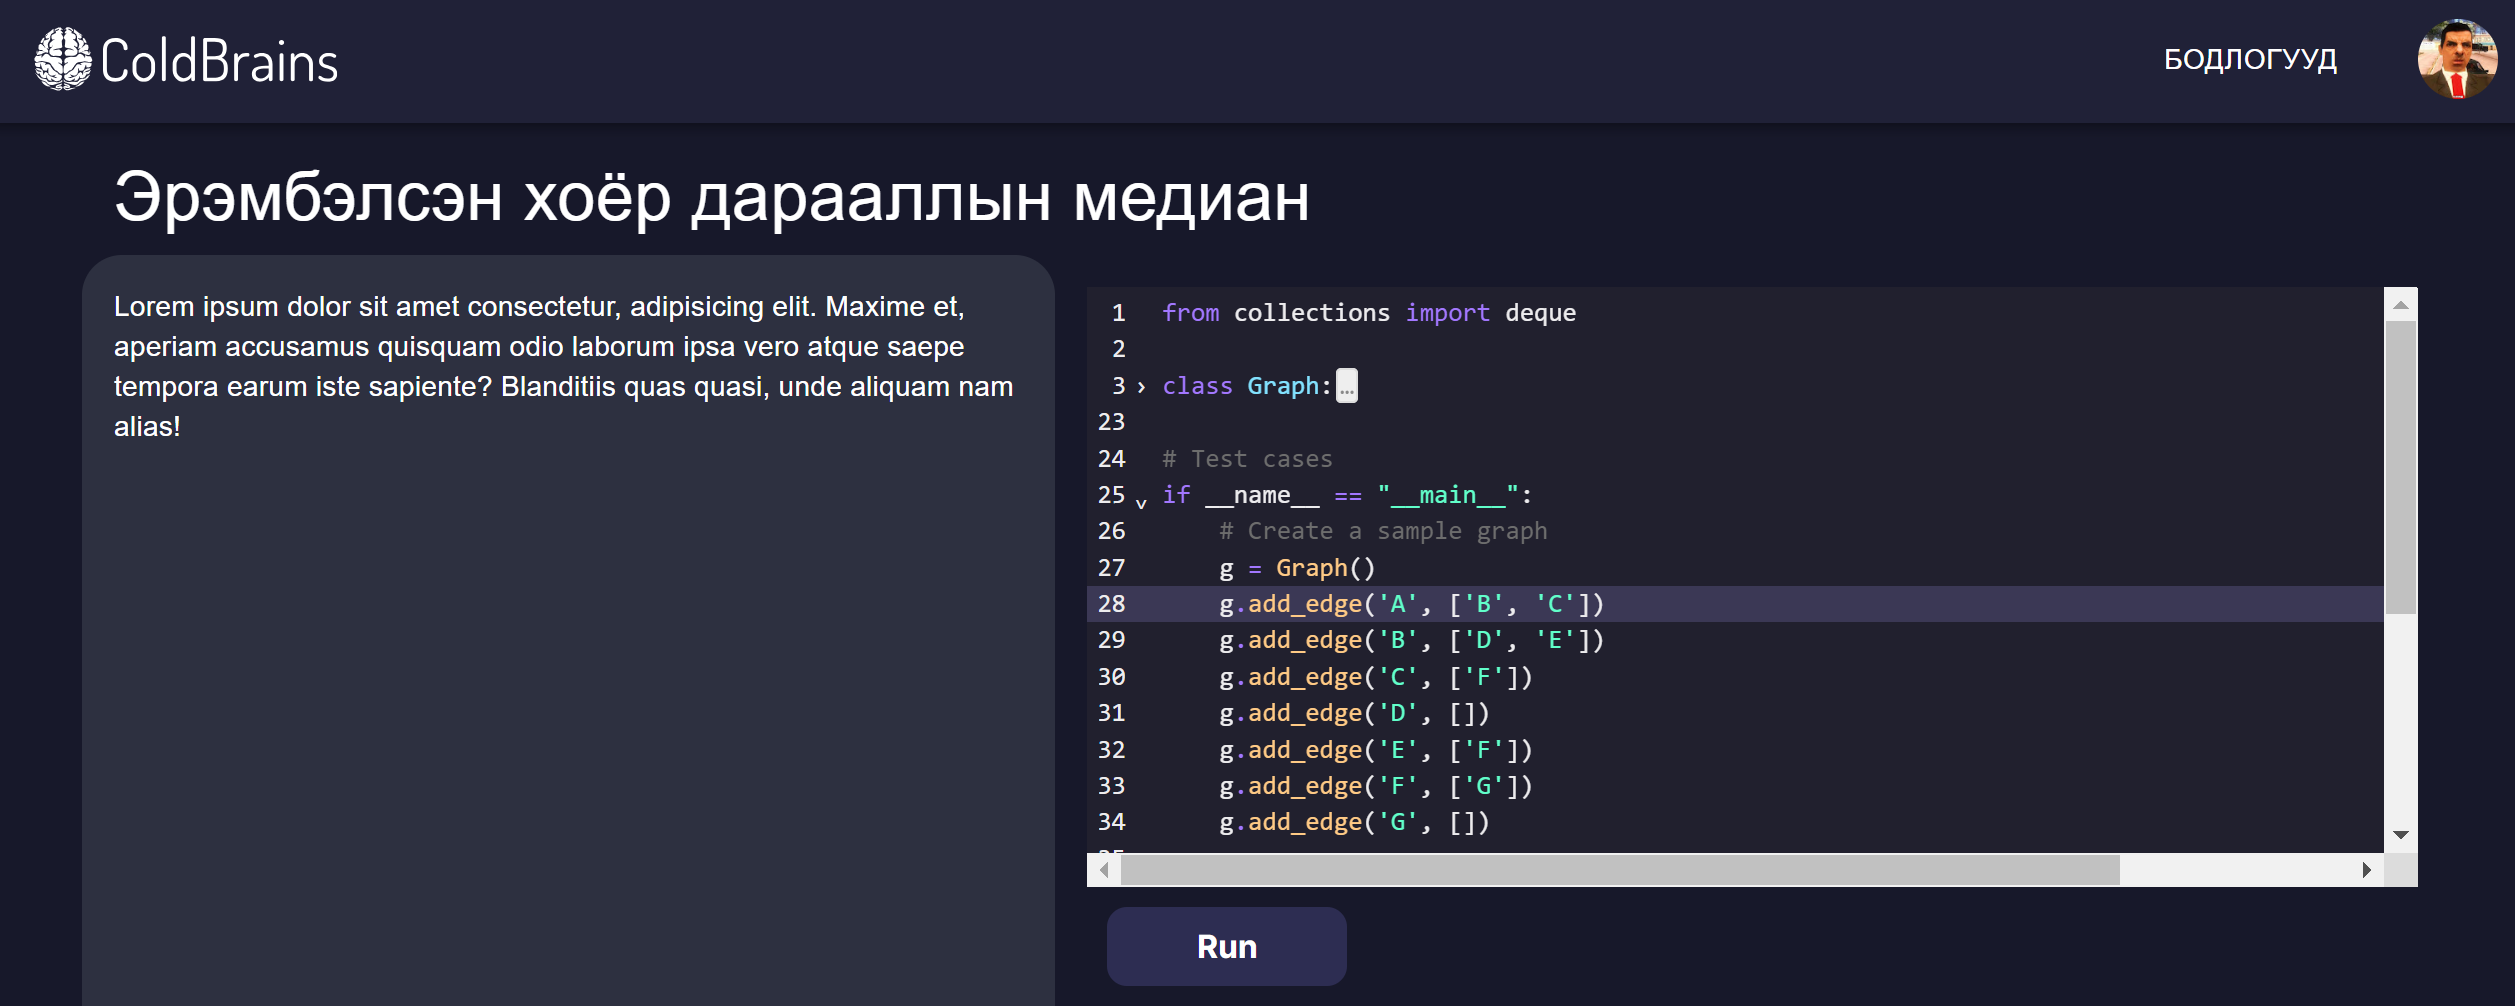
\includegraphics[width=16cm]{img/coldbrains-problem.PNG}
  \caption{Бодлого бодох хэсэг}
\end{figure}

\subsection{Session}
Хэрэглэгчийн бүртгүүлэх мэдээлэл болон нэвтрэх мэдээллийг өмнө дурьдсанчлан NEXTjs-ийн next-auth санг ашиглан хэрэгжүүлсэн бөгөөд хэрэглэгчийн мэдээлэл болох \textit{email}, \textit{Нэр}, \textit{Зураг} зэргийг үүсгэж session дээрээ JWT ашиглан encrypt хийх хэрэглэгч тал дээр cookie байдлаар хадгалж байгаа билээ. Энэхүү cookie нь next auth-ийн default behavior-оор 1 сар буюу 30 хоногийн хугацаатайгаар хэрэглэгчийн төхөөрөмж дээр оршино.

Хэрэглэгчийг бүртгэж авахдаа тухайн хэрэглэгчээс нэр, и-мейл, нууц үгийг авч байгаа бөгөөд хэрэглэгч талын middleware буюу NEXTjs middleware\cite{nextMid} дээр 
validation\footnotemark{} \footnotetext{Хэрэглэгчийн оролтыг баталгаажуулах процесс}-ийг хэрэгжүүлсэн байгаа билээ.

next auth сан болон firebase платформууд нь өөрсдийн гуравдагч платформуудын credentials provider-луу хандах боломжуудыг бий болгодог бөгөөд хэрэглэгч өөрийн и-мейл хаягийг хийн нэвтэрж орж буй тохиолдолд тухайн хэрэглэгчийн и-мейлийг баталгаажуулах процесс хийх нь шаардлагагүй гэж үзэв. Хэрэв тухайн хэрэглэгч энэхүү и-мейл хаягаар өөр платформ дээр ашигладаг бол "Coldbrains" системд бүртгэл үүсгэх шаардлагагүйгээр шууд нэвтрэх боломжтой билээ.

Хэрэглэгчийг тухайн хандах боломжтой эсэхийг системийн Frontend нь өөрийн сервер тал дээр тухайн хэрэглэгчийн session болох cookie-г decrypt хийн тогтмол шалгах бөгөөд тухайн хэрэглэгчийн session хугацаа нь дууссан, эсвэл мэдээлэл нь буруу байгаа тохиолдолд хэрэглэгчийг бүртгэлгүй хэрэглэгч гэж тооцон одоо хийж буй ажлын явцыг дуусгавар болгох боломжтой.

\subsection{Data fetching}
Хэрэглэгч нь Frontend рүү хүсэлт явуулах тоолонд сервер талаас өгөгдлийн сан руу хандах шаардлага бий болж байгаа билээ. Өгөгдлийн сангаас уншилт хийх аргыг хэдий оптимал байдлаар шийдсэн ч firestore нь өөрөө уншилт, бичилтүүдийн хязгаарлалтуудыг тавьж өгсөн тул системийн найдвартай ажиллагааны үүднээс тухайн уншилт бичилтүүдэд хязгаарлалт тавьж өгөх шаардлагатай. 

NEXTjs-ийн сервер талын route-үүд буюу тухайн route-үүд дээр firebase платформын админ SDK\footnotemark{} \footnotetext{Software Development Kit}-г ашиглан индекслэн document-үүд рүүгээ хандаж буй байдлаар хэрэгжүүлсэн. NEXTjs хувилбар 13 дээр шийдсэн javascript хэлний built-in \textbf{fetch(...)}\cite{NEXTcache} аргыг ашиглан сервер талдаа cache үүсгэж байгаа бөгөөд тухайн cache үүссэн тохиолдолд тэрхүү өгөгдлийг авах хүсэлт илгээж буй хэрэглэгчийн интерфейсүүд нь өгөгдлийн сангаас уншилт хийх шаардлагагүйгээр тухайн cache-ийг уншиж авна. 

Caching хийх нь Realtime өгөгдөлтэй харьцдаг системүүдийн хувьд тохиоромжгүй бөгөөд "Coldbrains" системийн хувьд бодлогын сан нь хэрэглэгч талдаа урт хугацаанд үл шинэчлэгдэх өгөгдөл гэж үзэн NEXTjs-ийн default хугацаа буюу 1 сарын хугацаатайгаар cache үүсгэж байгаа билээ. Харин идэвхитэй өөрчлөгдөх өгөгдөл буюу хэрэглэгчийн бодолтыг тухайн хэрэглэгчид realtime байдлаар харуулах шаардлага үүсч байна. Энэхүү тохиолдолд ерөнхий байдлаар caching хийх нь тохиромжгүй хэдий ч зардал багатайгаар шийдэх боломжууд мөн бий. Хэрэглэгчээс тухайн нөөцийг авах хүсэлт орж ирэх үед хамгийн боломжит богино интервалтайгаар cache үүсгэх боломжтой бөгөөд тухайн cache-ийг 3 секундын хугацаатайгаар хэрэгжүүлснээр богино хугацаанд орж ирэх зэрэгцээ хүсэлтүүдэд computing\footnotemark{} \footnotetext{Тооцоолж, боловсруулах процесс} хийх нөөцийг хэмнэх юм. 

86400секунд/өдөр : 3секунд/уншилт = 28800уншилт/өдөр болох бөгөөд хэрэгцээт уншилтуудын хязгаарт хэдэн ч хэрэглэгч байсан багтаах боломжтой болж байгаа юм.

3 секундын интервалиар тохируулж өгөх нь бодолгоо дөнгөж бодож буй хүнд эргээгээд бодолтуудыг харуулах нь илүү урт хугацаа мэт байгаа боловч зэрэгцээ тухайн хэрэглэгчээс өмнө 3 секунд дотор өөр хэрэглэгч ижил бодлогыг бодож cache үүсгэх нь ховор тохиолдол бөгөөд дараачийн хэрэглэгч нь тухайн хуудсыг дахин ачааллуулах нь UX-д ашиглагддаг түгээмэл практикуудын нэг юм.

\begin{figure}[H]
  \centering
  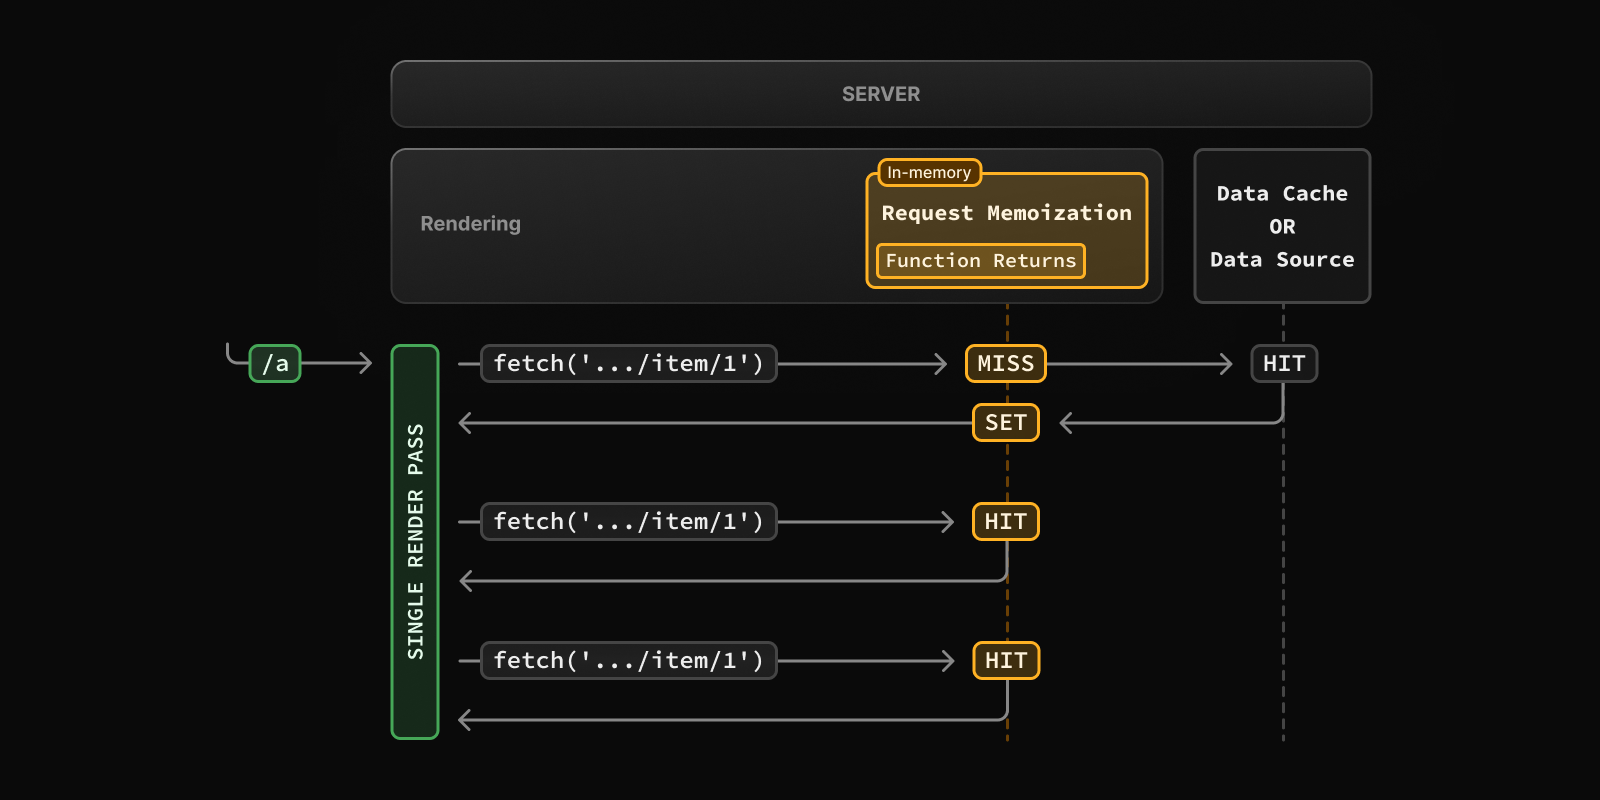
\includegraphics[width=10cm, height=4cm]{img/request-memo.png}
  \caption{NEXTjs-ийн сервер талдаа cache ашиглаж буй байдал}
\end{figure}
\clearpage

\subsection{Code editor}
Технологиуд дээр дурьдсанчлан хэрэглэгчийн кодыг засварчлахдаа \textbf{Codemirror} javascript хэлний санг ашигласан бөгөөд тухайн санг React дээр интеграц хийж илүү олон боломжуудтайгаар ашиглахын тулд \textbf{@uiw/react-codemirror} санг ашигласан билээ. Өнгөний сонголт, түгээмэл код засварлагчийн theme-үүдийг түүний өргөтгөл сан болох \textbf{@uiw/codemirror-themes-all} санг ашигласан. Энэхүү сан нь React дээр бэлтгэж өгсөн код засварлагч копмонентээр хангаж өгдөг бөгөөд тухайн код засварлагч дээр customize буюу өөрөө гараар бичсэн өргөтгөл функцуудыг нэмэх боломжтой. Системд ашиглахдаа өөр бусад Tern.js зэрэг ухаалаг санал болгогч төлөвлөсөн байгаа бөгөөд одоогоор бодлого бодох үед хэрэглэгчид ухаалгаар санал болгогч ашиглуулах нь хэрэглэгчид хэтэрхий хялбарчилж өгч байсан тул хэрэглэгчийн суурь мэдлэгийг бататгах үүднээс системийн бодлого бодох хэсэгт нэмээгүй байгаа билээ.

Одоогоор python хэлний код ажлуулагч серверийг validation, sandboxing зэргээр хэрэгжүүлсэн байгаа билээ. Үүнд зориулан python хэлэн дээр хэрэглэгчид boilerplate кодыг анх тайлбартайгаар үүсгэж өгч байгаа бөгөөд хэрэглэгчийн тухайн кодыг хэрхэн ашиглаж програмын оролтыг ашиглахыг зөвлөсөн байгаа юм. 

\begin{figure}[H]
  \centering
  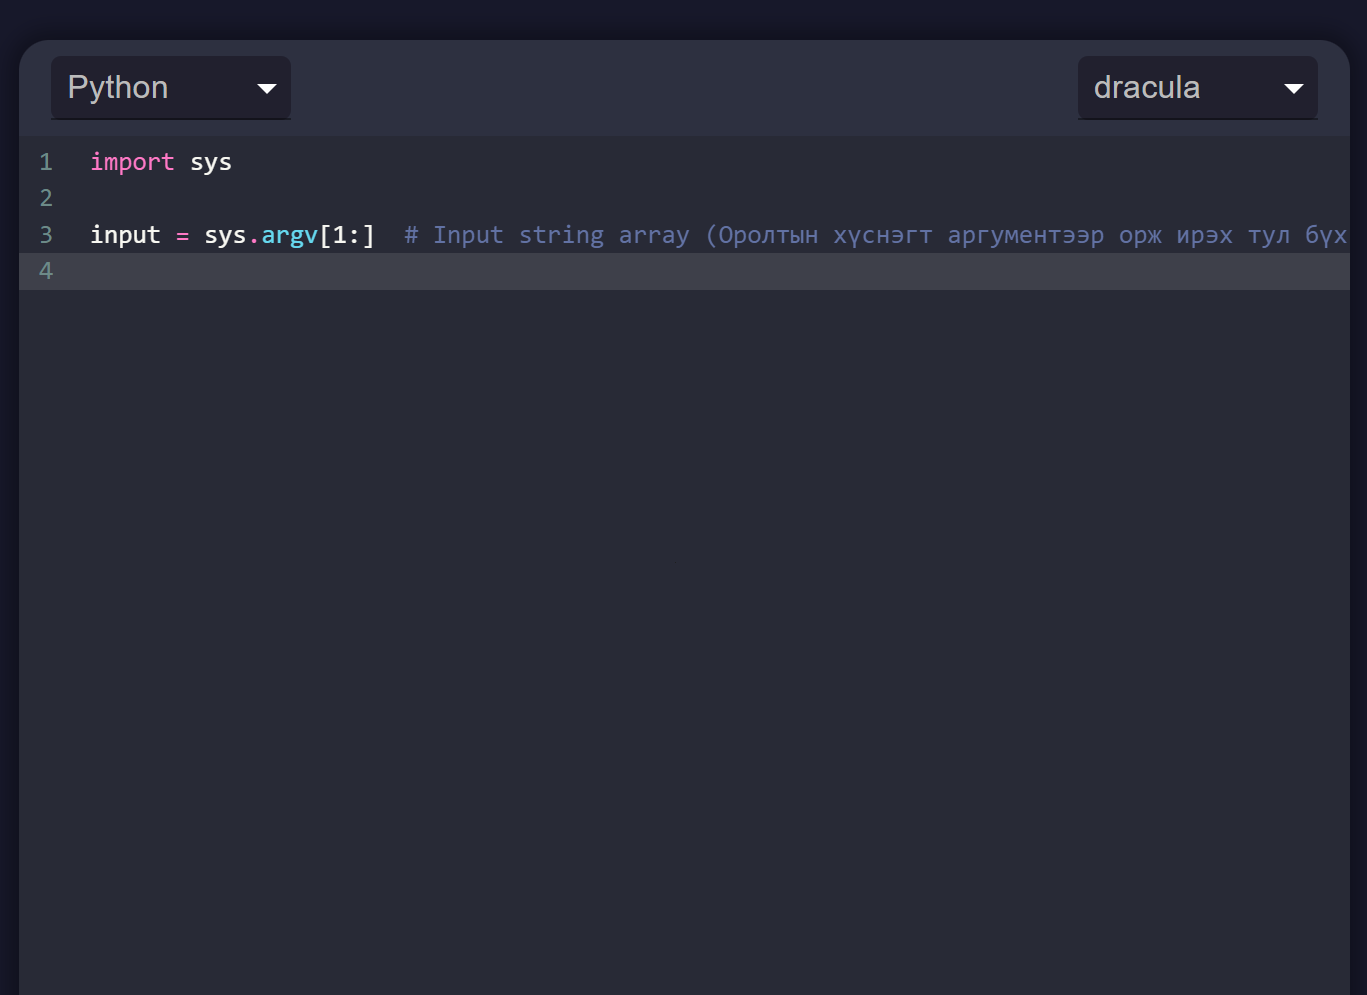
\includegraphics[width=10cm]{img/testEditor.PNG}
  \caption{Dracula theme дээр python хэлний boilerplate бүхий код засварлагч}
\end{figure}

\begin{figure}[H]
  \centering
  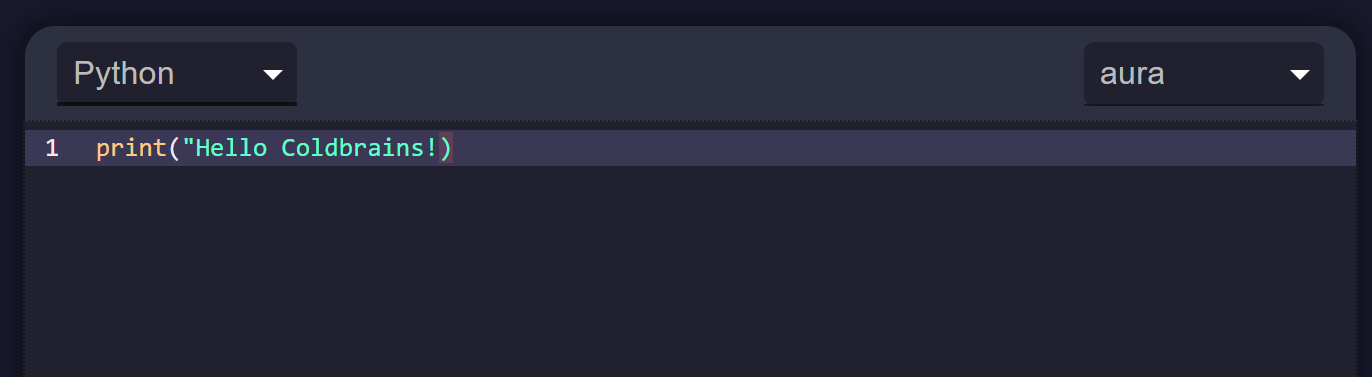
\includegraphics[width=10cm]{img/syntaxErr.PNG}
  \caption{Syntax-ийн алдаа бүхий код}
\end{figure}

\begin{figure}[H]
  \centering
  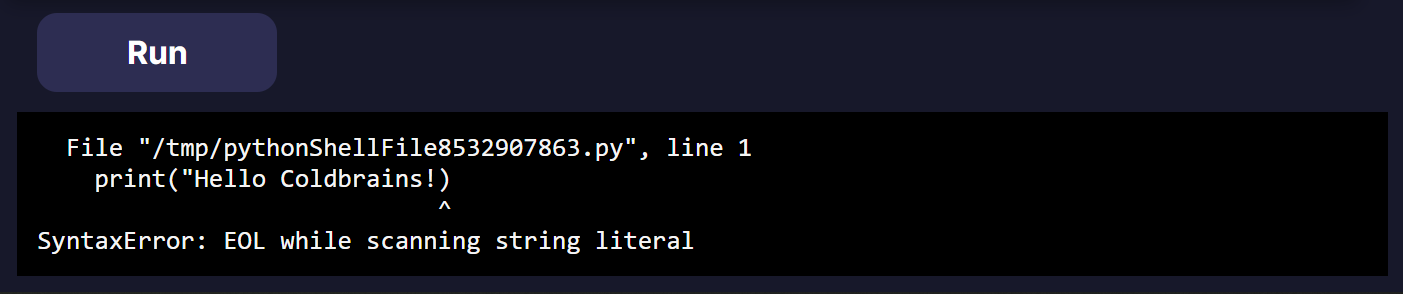
\includegraphics[width=10cm]{img/syntaxErrOut.PNG}
  \caption{Syntax-ийн алдааг харуулж буй системийн интерфейс}
\end{figure}

Эдгээр хэрэглэгчийн коднууд нь -> NEXTjs сервер -> ExpressJS сервер -> Coderunner сервер зэрэг байдлаар дамжин ажиллуулж эргээд Coderunner -> ExpressJS  сервер-> NEXTjs сервер -> интерфейс гэх дарааллаар хариугаа хэрэглэгчид харуулж байгаа юм. 

\begin{figure}[H]
  \centering
  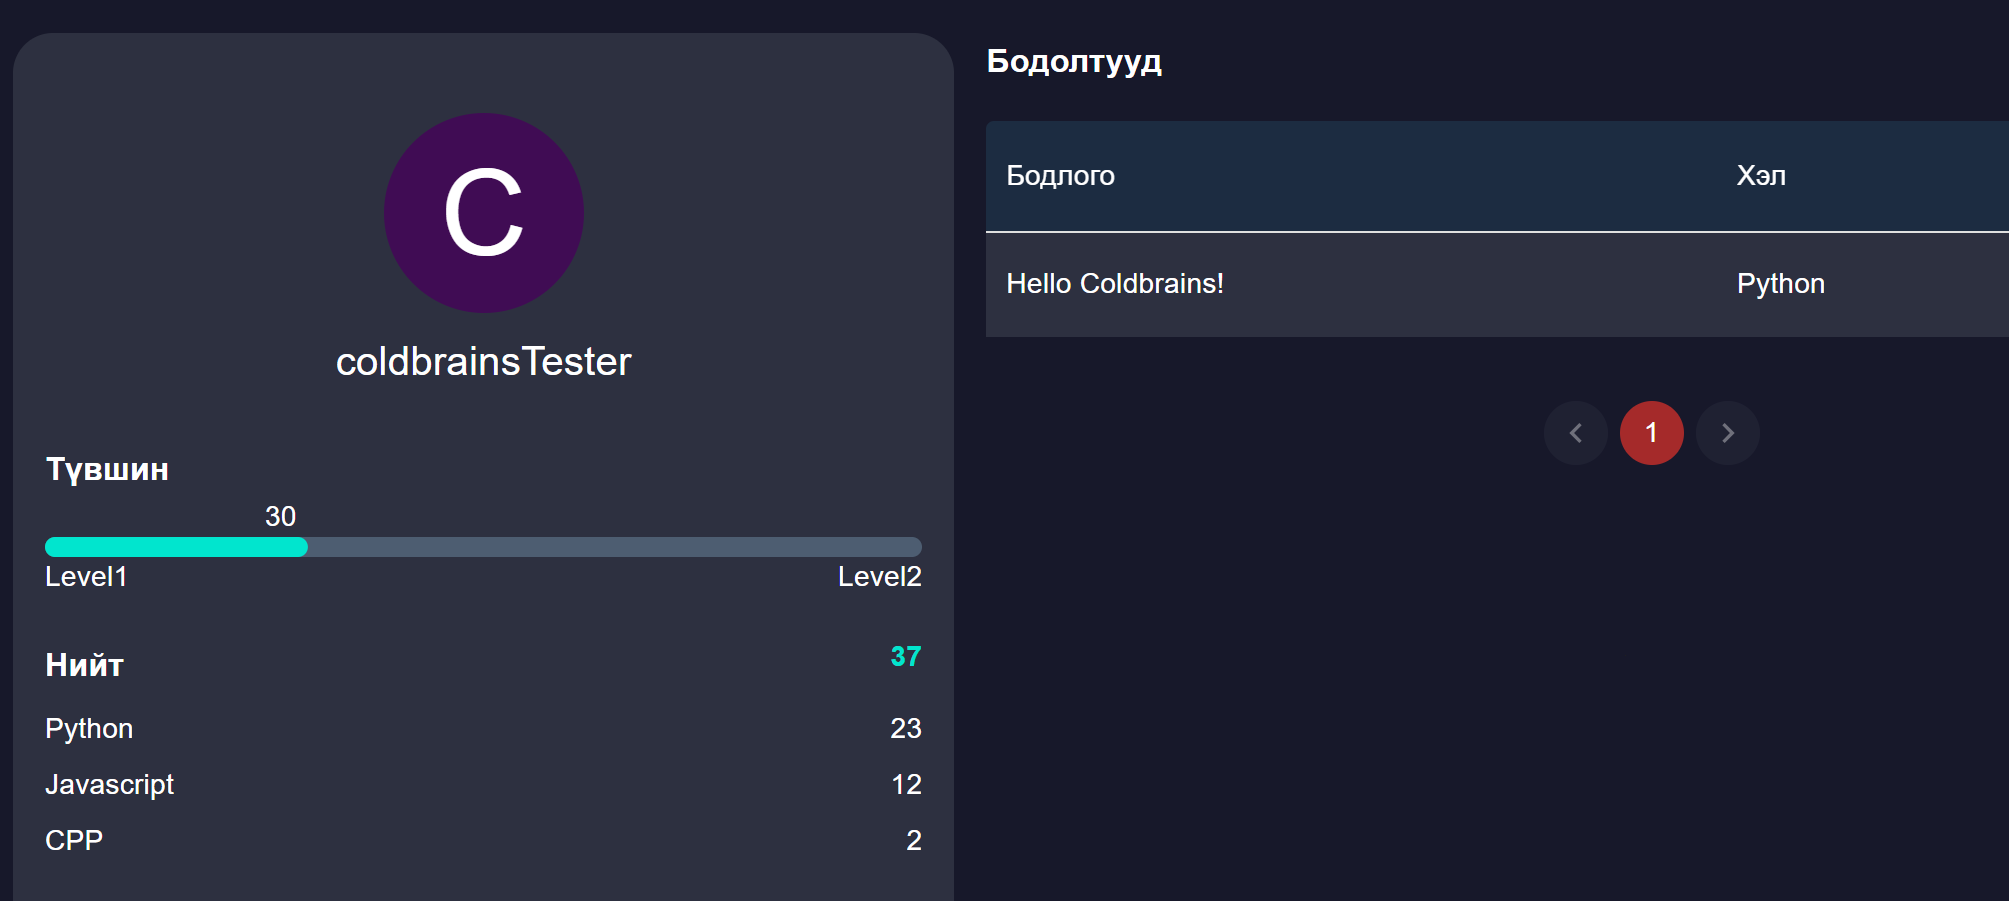
\includegraphics[width=12cm]{img/profileImp.PNG}
  \caption{Хэрэглэгчийн профайл хуудас}
\end{figure}

\clearpage
\section{Backend}
Хэрэглэгчийн нууц үгийг hash-лах bcrypt ашиглан, auth серверийг MySQL дээр тест байдлаар хэрэгжүүлсэн байгаа бөгөөд ExpressJS дээр modular-programming техникийг ашиглаж байгаа билээ. Одоогоор хэрэглэгчийн кодыг Python-shell дээр ажиллуулах, хэрэглэгчийг бүртгэх, нэвтрэх, request throttling хийх зэрэг ажлуудыг гүйцэтгээд байгаа билээ.

\begin{figure}[h]
  \centering
  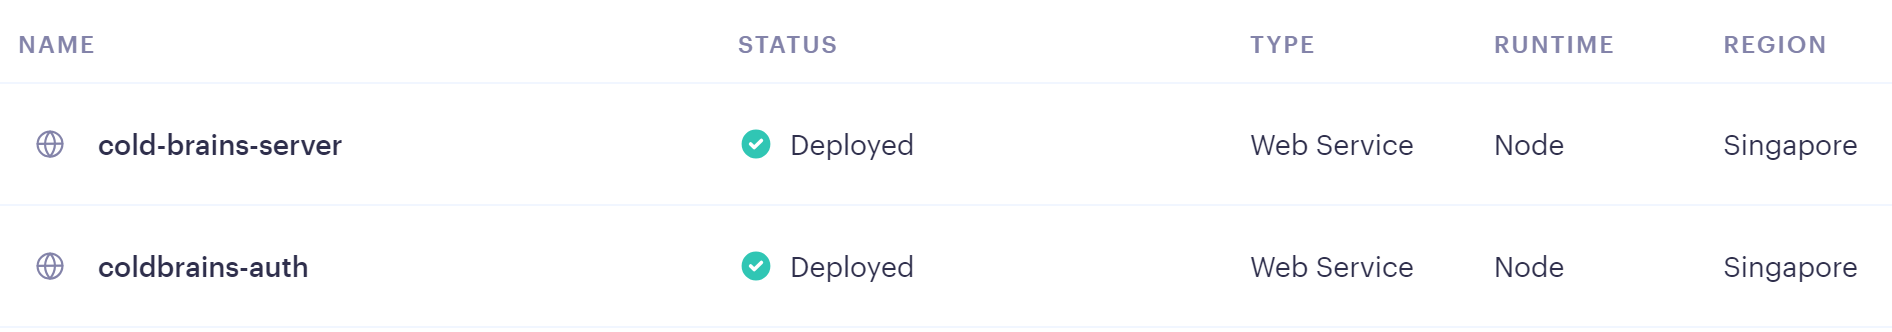
\includegraphics[width=16cm]{img/render.com.png}
  \caption{Сервисүүдийг байршуулсан байдал}
\end{figure}

Зохиомжийн дагуу хэрэглэгчийн кодыг дүгнэх процессийг хэрэгжүүлсэн бөгөөд ExpressJS-ийн middleware-уудыг ашиглан хэрэглэгчээс орж ирэх хүсэлтүүдийг шүүж хязгаарлаж өгсөн билээ.

\subsection{Middleware}
\textbf{express-rate-limit} санг ашиглан хэрэглэгчийн хандалтад хязгаар тавьж өгсөн бөгөөд одоогоор 5 секундэд 5 удаа хандах боломжтой байлгаж хязгаарласан байгаа билээ. Хязгаарлалтыг тавьж өгснөөр Coderunner серверийн нөөцийг хэрэггүй зүйлд ашиглахаас сэргийлж байгаа бөгөөд brute-force болон бусад өөр зорилго агуулсан хандалтаас сэргийлэх боломжтой. 

expressJS дээр цаашлаад ирж болон хүсэлтийн payload буюу body датаг хязгаарлалт хийн шийдэж өгч байгаа. ExpressJS сервер нь хэрэглэгчээс бодолтыг авч тухайн бодолтын тест кейсүүдийг firestore-оос уншиж цааш Coderunner луу дамжуулах үүрэг хүлээж байгаа бөгөөд хэрэглэгчээс орж ирэх кодын хэмжээг хязгаарлах, мөн хаанаас ирэх хаягийг CORS ашиглан блоклож байгаа юм. Хэрэглэгчийн кодын хэмжээ нь бодлого бодох хэмжээнээс хэтэрч ямар нэгэн гуравдагч санг хэрэгжүүлсэн тохиолдолд кодын хэмжээгээр хязгаарлах байдлаар шийдсэн.

\subsection{Coderunner}
\textbf{python-shell} санг ашиглан тухайн ирж буй кодыг ажиллуулахыг AWS Lambda сервертэй цогцоор нь шийдсэн. Тухайн код их хэмжээний нөөцийг ашиглах, тухайн төхөөрөмжийг улмаар хэвийн ажиллагааг зөрчилдүүлсэн тохиолдолд AWS Lambda сервер нь cold boot хийн stateless учир ямарваа нэгэн өмнөх ажилласан мэдээллээ хадгалахгүйгээр дахин шинээр ажиллаж эхлэх билээ.

Өөр нэгэн шийдэл бол container технологийг өөрөө хэрэгжүүлэн тухайн container-т CPU, RAM зэрэг computing нөөцүүдийг хязгаарлаж, сүлжээнд хандах болон бусад сүлжээ рүү хариулахаас сэргийлэх боломжтой. Энэ нь энгийн бөгөөд үр дүнтэй ажиллах боломжтой арга билээ. Хөгжүүлэлт болон тохиргооны хувьд ихээхэн зардал гарах боломжтой бөгөөд тухайн Coderunner серверийг багцлан container-ийг үүсгэсэн тохиолдолд
эдгээр коммандуудыг ажиллуулан тухайн серверийн Sandboxing, Network restriction зэрэг асуудлуудыг шийдэх боломжтой.

\begin{figure}[H]
  \centering
  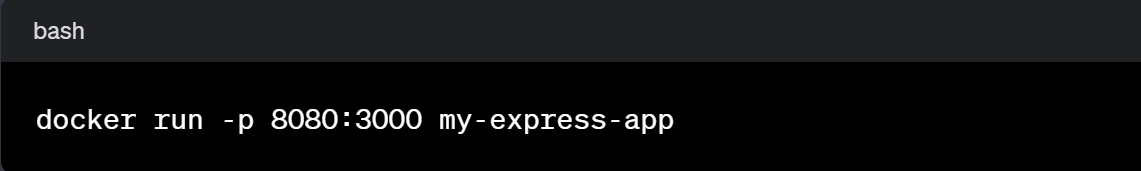
\includegraphics[width=12cm]{img/docker-port.PNG}
  \caption{Хандах боломжтой портыг тодорхойлох}
\end{figure}

\begin{figure}[H]
  \centering
  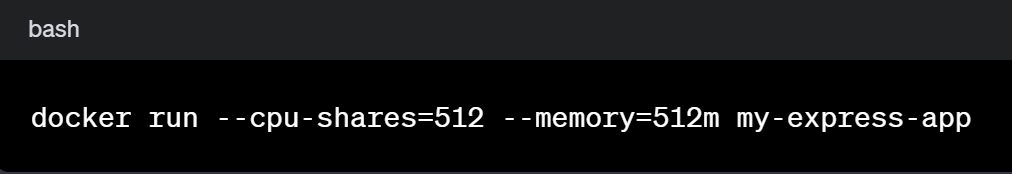
\includegraphics[width=12cm]{img/docker-resource.PNG}
  \caption{Нөөцийг хязгаарлах}
\end{figure}

\begin{figure}[H]
  \centering
  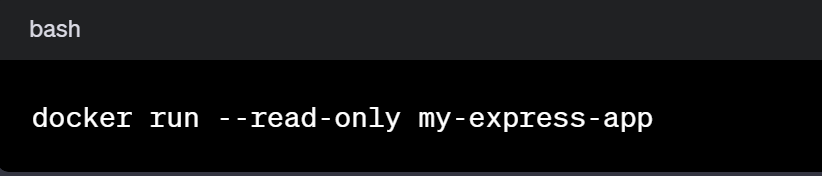
\includegraphics[width=12cm]{img/docker-readonly.PNG}
  \caption{Зөвхөн унших боломжтой болгох}
\end{figure}

Энэхүү шийдэл нь зэрэгцээ хандалт болон тухайн скрийптийг хэрхэн хувааж хэрэглэх болон бусад олон асуудлуудыг бий болгох бөгөөд илүү enterprise түвшний хөгжүүлэлтүүдийг шаардах билээ.
"Coldbrains" системийн хувьд MVP-г зорьсон бөгөөд AWS Lambda ашигладаг Render платформ дээр container болгон Coderunner серверийг байршуулсан байгаа юм. Уг шийдэл нь дээр дурьдсан шийдлээс илүү болхи хэдий ч зардал багатай, чанарын үзүүлэлтүүдээр дүйцэхүйц байгаа билээ.

Уг шийдэл дээр Python програмчлалын хэлний built-in сүлжээнд ажиллах, файл системд нэвтрэх, үйлдлийн системд бичих сангуудыг блоклож байгаа бөгөөд үүнийг \textit{regex} ашиглан хэрэглэгчийн кодноос тухайн сангуудын ашиглалтад хайлт хийдэг middleware байдлаар хэрэгжүүлсэн.

\subsection{Байршуулалт, ашиглалт}
Render платформын AWS Lambda серверүүдийг ашиглаж байгаа бөгөөд идэвхигүй болсон үедээ \textbf{spin down} хийдэг энэхүү серверүүд нь эргээд асах буюу \textbf{cold boot} хийхдээ анх build хийхэд байсантайгаа ижил төлөвт ордог билээ\cite{renderfree}. Spin down хийсэн container-үүд нь энэхүү Render платформын төлөвлөгөөнд эргээд 10-15 секунд асахад зарцуулдаг гэж заасан. Сүлжээнд алдах цагийг багасгах зорилгоор Coderunner сервер болон ExpressJS серверүүдийг тус бүрийг нь Render платформ дээр байршуулсан бөгөөд хоорондоо local орчинд шууд харилцан датагаа богино хугацаанд дамжуулах боломжтой билээ. Сүлжээнд тест кейс болон хэрэглэгчийн кодыг дамжуулах нь ихээхэн хугацаа шаардах бөгөөд хамтад нь Singapore дээрх инстанци дээр байршуулав. 

Хэрэглэгчээс ирэх дата нь эхэлж ExpressJS-ийг cold boot хийлгээд тухайн cold boot хийсэн container нь дахин CodeRunner-ийг асаана. Энэ нь хүлээлгийн араас хүлээлэг үүсгэн \textit{GATEWAY TIMEOUT 504} алдааг хэрэглэгчид харуулахад хүргэх бөгөөд нийт 40-45 секунд хугацааг код ажиллуулах хүсэлт боловсруулахад зарцуулж байгаа билээ. Үүнийг шийдсэн арга нь тухайн 2 container-ийг зэрэгцээ cold boot хийлгэсэн бөгөөд код ажиллуулах хүсэлт явуулахдаа NEXTjs route middleware-ээс тухайн Coderunner container лүү ping хийж нийт 10-15 секунд cold boot хийхэд зарцуулж байгаа билээ. 

Цаашлаад stateless байдлаар кодыг зохиомжилсон бөгөөд санах ой дээр үүсдэг ямарваа нэгэн тогтмол ашиглагдах инстанциудыг cold boot хийх үед дахин үүсгэх байдлаар програмчилж бичив.

\subsection{Firestore}
Frontend болон Backend тус бүр Firebase admin SDK ашиглан query бичин байгаа бөгөөд тухайн query-г хурдацтай ажиллуулахын тулд collectionGroup үүсгэн тухайн бодлогын бодолтууд болон хэрэглэгчийн бодолтуудыг богино хугацаанд авах боломжтой болгосон билээ.

\begin{figure}[H]
  \centering
  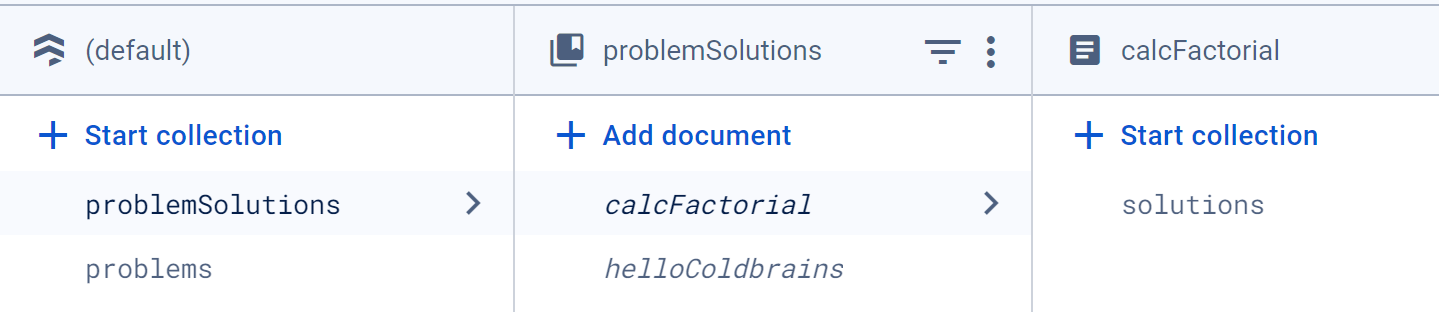
\includegraphics[width=12cm]{img/firestore1.PNG}
  \caption{Firestore-ийн ProblemSolutions collection болон түүний заагч document-үүд}
\end{figure}

\begin{figure}[H]
  \centering
  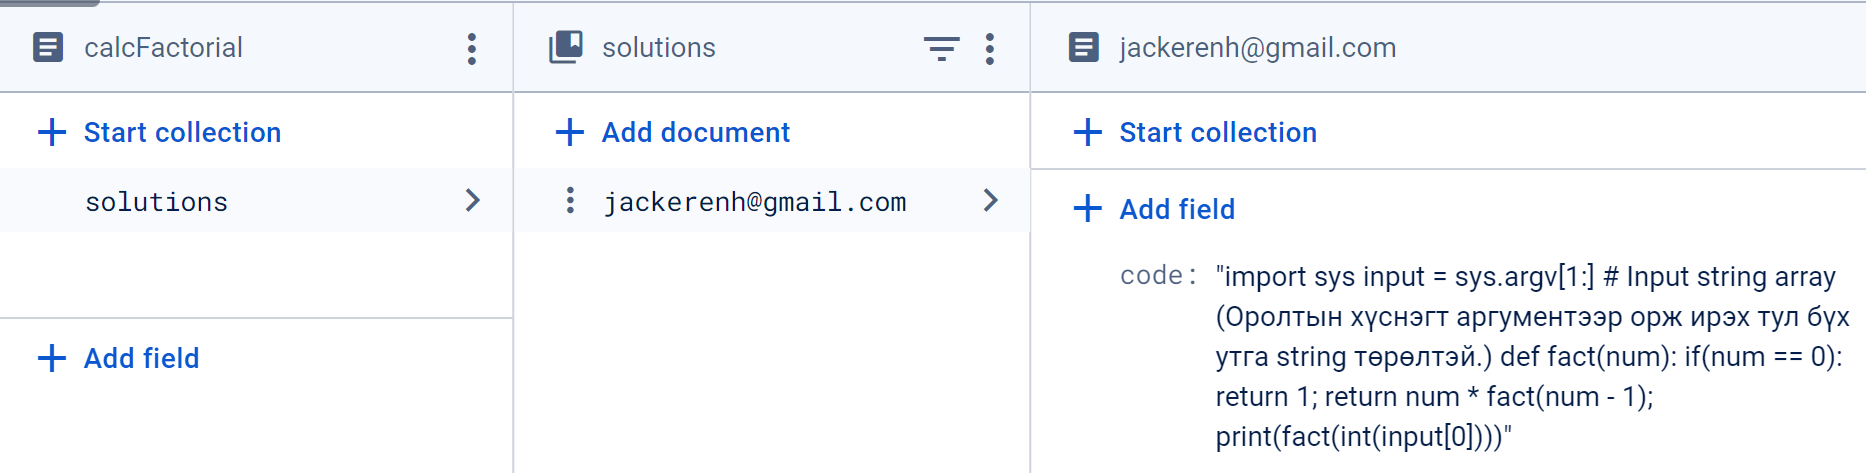
\includegraphics[width=12cm]{img/firestore2.PNG}
  \caption{Firestore-ийн subcollection group-ийн ашиглалт, агуулж буй document-үүд}
\end{figure}